Consider the wave equation
\[ u_{tt}(x,t) = u_{xx}(x,t) \]
for $0\le x\le 1$ and $t\ge 0$ subject to the \emph{mixed} boundary conditions
\[ u(0,t) = 0, \qquad {\d u\over \d x}(1,t) = 0\]
for all $t\ge 0$ and initial conditions
\[  u(x,0) = u_0(x) = \sum_{n=1}^\infty a_n(0) \psi_n(x), \qquad
    u_t(x,0) = v_0(x) = \sum_{n=1}^\infty b_n \psi_n(x),\]
where the functions $\psi_n$ are the eigenfunctions 
\[ \psi_n(x) = \sqrt{2} \sin(\sqrt{\lambda_n}@x)\]
of the operator
   \[ L u = -u_{xx}\]
with initial conditions $u(0) = u_x(1) = 0$  and 
eigenvalues $\lambda_n = (n-1/2)^2 \pi^2$ for $n=1,2,\ldots.$\\
(Recall that you computed these eigenvalues and eigenfunctions on Problem Set~5.)


%%%%%%%%%%%%%%%%%%%%%%%%%%%%%%%%%%%%%%%%%%%%%%%%%%%%%%%%%%%%%%%%%%%%%%%%%%%%%%%%

\begin{enumerate}
\item We wish to write the solution to this wave equation in the form
         \[ u(x,t) = \sum_{k=1}^\infty a_k(t) \psi_k(x).\]
      Show that the coefficients $a_k(t)$ obey the ordinary differential equation 
       \[ a_k''(t) = -\lambda_j a_k(t) \]
      subject to the initial values $a_k(0)$ and $a_k'(0) = b_k(0)$
      obtained from $u_0$ and $v_0$.

\item Write down the solution to the differential equation in part~(a).

\item Use your solution to part~(b) to write out a formula for the solution $u(x,t)$.

\item Write a MATLAB program to compute solutions to this differential equation 
      with initial conditions
        \[ u_0(x) = 0, \qquad v_0(x) = x+\sin(\pi x).\]
      Submit your code, along with a surface plot showing the solution over 
      the spatial interval $x\in[0,1]$ and the time interval $t\in [0,10]$.
\end{enumerate}

%%%%%%%%%%%%%%%%%%%%%%%%%%%%%%%%%%%%%%%%%%%%%%%%%%%%%%%%%%%%%%%%%%%%%%%%%%%%%%%%

\ifthenelse{\boolean{showsols}}{\begin{solution}

\begin{enumerate}
\item If we write the solution in the form
         \[ u(x,t) = \sum_{j=1}^\infty a_j(t) \phi_j(x)\]
      for any $t\ge 0$, and substitute this series into the differential equation,
      we obtain
         \[ \sum_{j=1}^\infty {d^2 a_j \over dt^2}(t) \phi_j(x)
               = c^2 \sum_{j=1}^\infty a_j(t) {d^2 \over dx^2} \phi_j(x).\]
      Since $\phi_j$ is an eigenfunction of the operator $L$, we simply have
         \[ \sum_{j=1}^\infty {d^2 a_j \over dt^2}(t) \phi_j(x)
               = -c^2 \sum_{j=1}^\infty a_j(t) \lambda_j \phi_j(x).\]
      Take the inner product of both sides with $\phi_k$ and use the 
      orthogonality of the eigenfunctions to obtain
         \[ {d^2 a_j \over dt^2} (t) = -c^2 \lambda_j a_j(t).\]
      At time $t=0$, we have
\[  u(x,0) = \psi(x) = \sum_{n=1}^\infty b_n \phi_n(x), \qquad
    {\d u \over \d t}(x,0) = \gamma(x) = \sum_{n=1}^\infty d_n \phi_n(x),\]
      which we can compare with the expansion
\[ u(x,0) = \sum_{j=1}^\infty a_j(0) \phi_j(x), \qquad
 {\d u \over \d t}(x,0) = \sum_{j=1}^\infty {d a_j \over d t}(0) \phi_j(x)\]
to identify the initial conditions
\[  a_j(0) = b_j, \qquad {\d u \over \d t}(x,0) = d_j.\]

\item The differential equation derived in part~(a) has a general solution
      of the form
\[ a_j(t) = A \sin(c\sqrt{\lambda_j} t) + B \cos(c\sqrt{\lambda_j} t).\]
The constants $A$ and $B$ are determined by the boundary conditions.
At $t=0$, the above formula takes the value
\[ a_j(0) = A \sin(0) + B \cos(0) = B.\]
Hence we conclude that 
\[ B = b_j.\]
The derivative of our formula for $a_j$ gives
\[ {d a_j \over d t}(0) = c \sqrt{\lambda_j} A \cos(0) + c \sqrt{\lambda_j} B \sin(0) 
                        = c \sqrt{\lambda_j} A,\]
and since we require $(d a_j/dt)(0)=d_j$, we have
\[ A = {d_j\over c \sqrt{\lambda_j}} = {d_j \over c (j-1/2) \pi}.\]
Thus we have
\[ a_j(t) = \Big({d_j \over c (j-1/2)\pi}\Big) \sin(c \sqrt{\lambda_j} t) 
              + b_j \cos(c \sqrt{\lambda_j} t).\]


\item With this formula for $a_j(t)$, we can write down the full solution
to the differential equation
\[ u(x,t) = \sum_{j=1}^\infty \Big[\Big({d_j \over c (j-1/2)\pi}\Big) 
                   \sin(c \sqrt{\lambda_j} t) + b_j \cos(c \sqrt{\lambda_j} t)\Big]
                    \big(\sqrt{2} \sin(\sqrt{\lambda_j} x)\big).\]
         
\item MATLAB code to solve this problem with $c=1$ is included below.  
      Since $u(0,t) = 0$ we have  $b_j = 0$.  
      We can use Mathematica or MATLAB to compute the $d_j$ that give
      \[ {\d u \over \d t}(0,t) = x+\sin(\pi x) = \sum_{j=1}^\infty d_j \phi_j(x).\]
      In particular, since the eigenfunctions are normalized, we have
      \begin{eqnarray*}
         d_j = (x + \sin(\pi x), \phi_j) 
            &=& {4\sqrt{2} (-1)^{j}\over \pi^2}
                 \Big({\pi \over 4j^2-4j-3} - {1\over (1-2j)^2}\Big) \\[0.5em]
            &=& \sqrt{2} (-1)^{j+1}
                \Big({1\over \lambda_j} + {\pi \over \pi^2 -\lambda_j}\Big).
      \end{eqnarray*} 
      The solutions at times $t=0, 0.5, 1.0, 1.5, 2.0$ are shown in the plots below.

\begin{center}
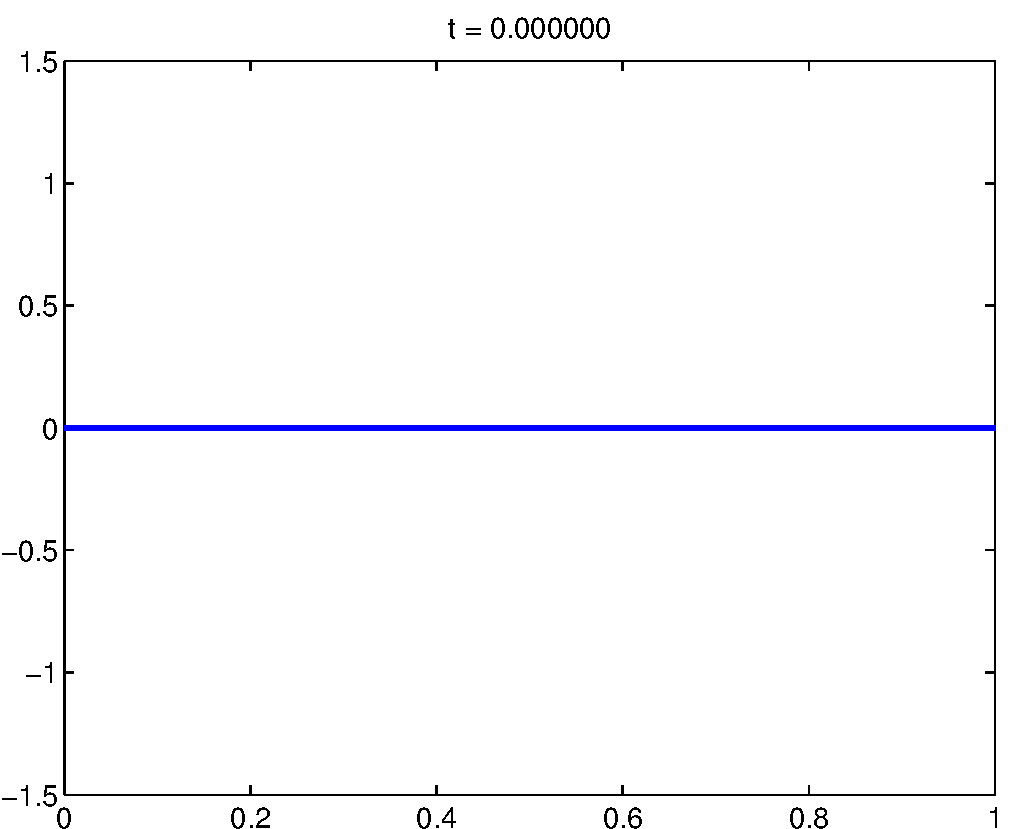
\includegraphics[scale=0.35]{mixed_0}\quad
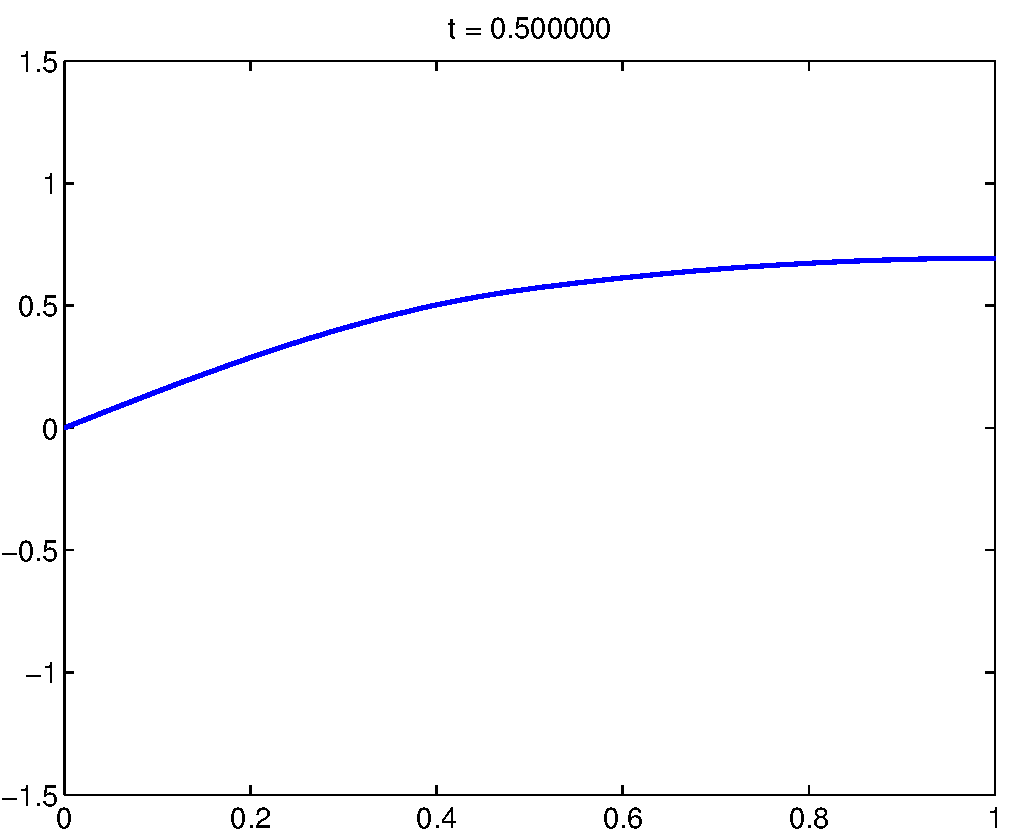
\includegraphics[scale=0.35]{mixed_1}

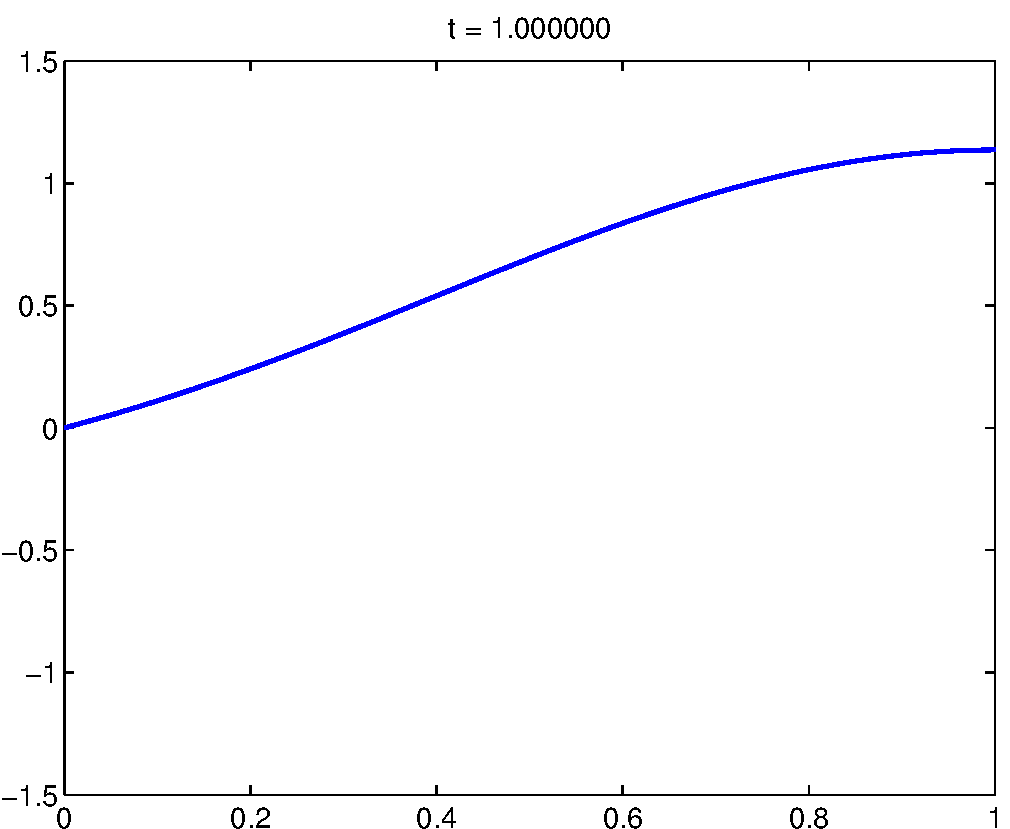
\includegraphics[scale=0.35]{mixed_2}\quad
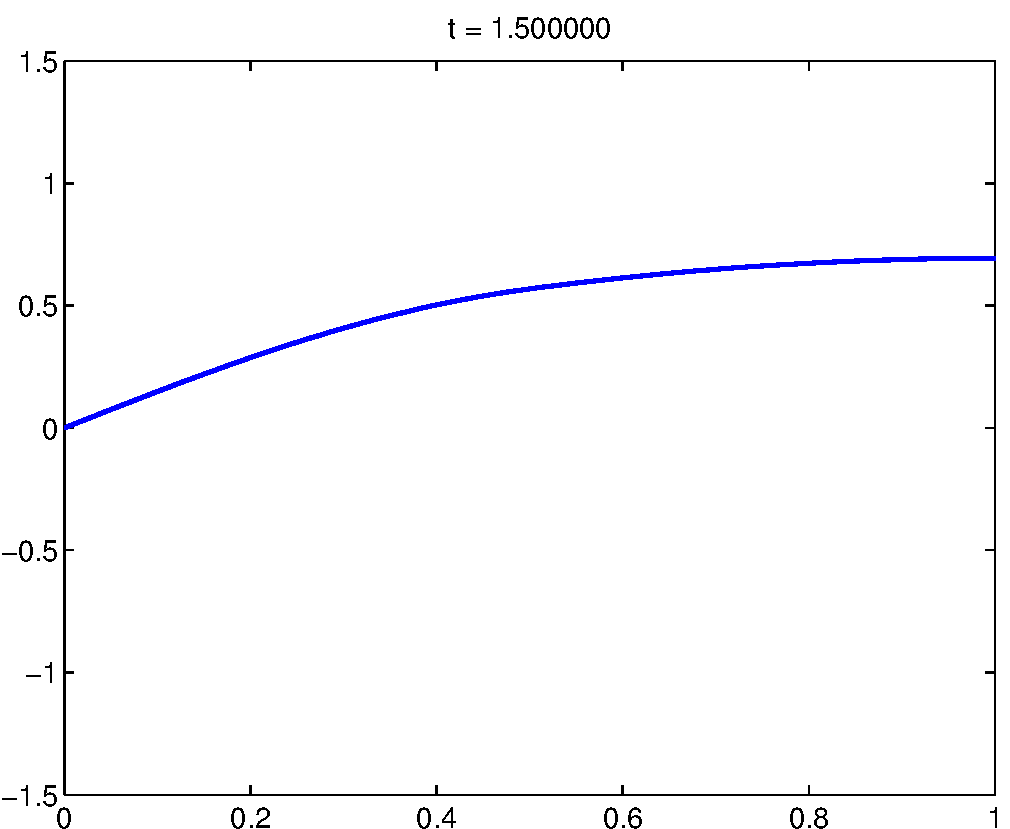
\includegraphics[scale=0.35]{mixed_3}

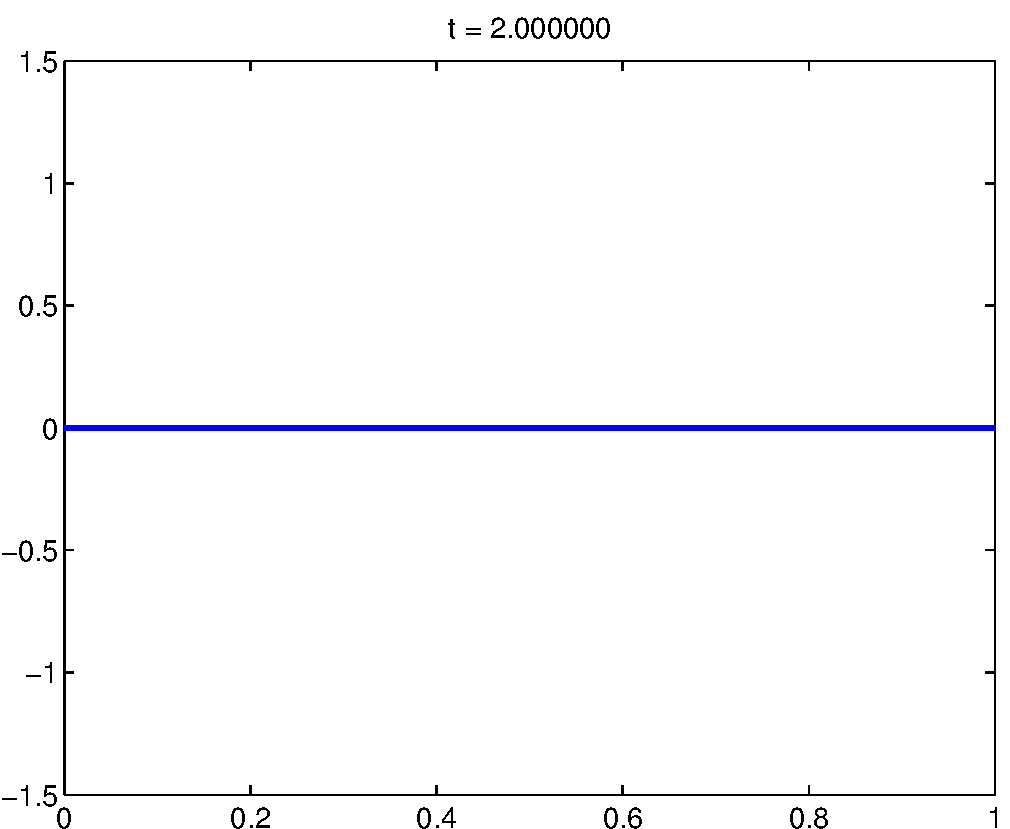
\includegraphics[scale=0.35]{mixed_4}
\end{center}

These plots are rather boring, so we also show the action in three dimensions.

\begin{center}
   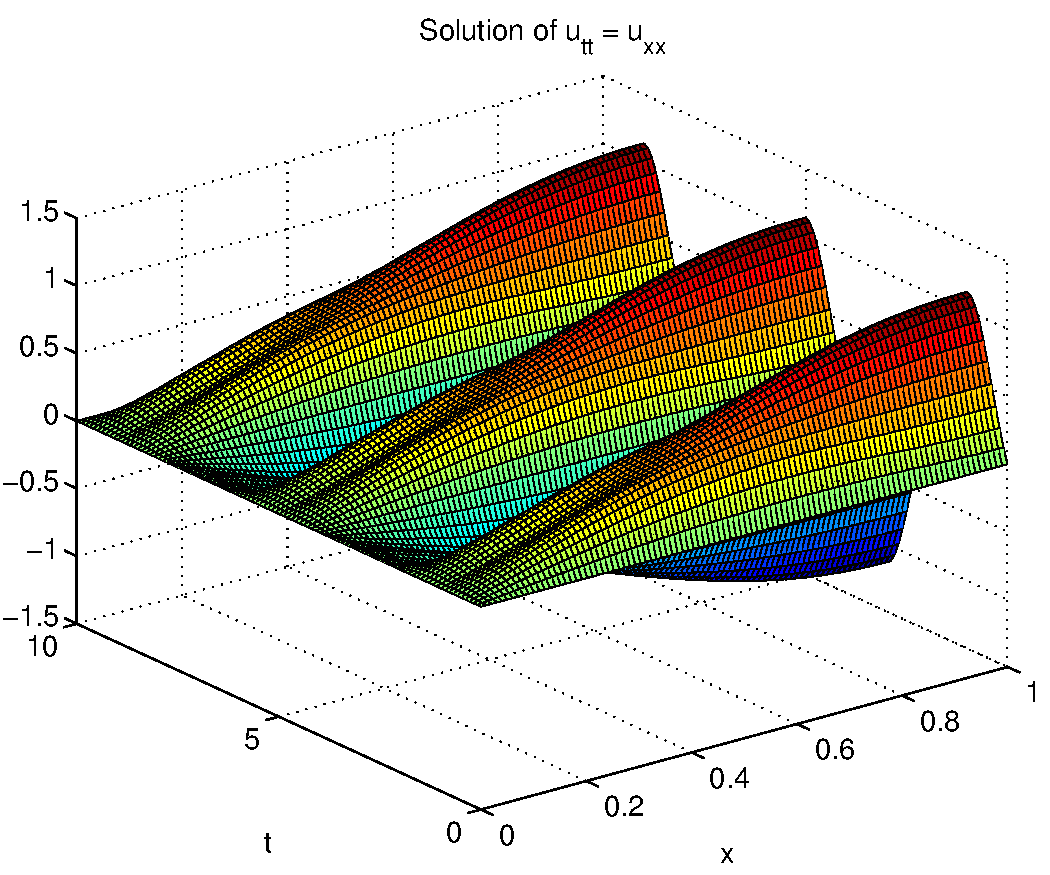
\includegraphics[scale=0.55]{mixed_3d}
\end{center}
\end{enumerate}

\input mixed_code
\end{solution}}{}

